
\documentclass[12pt]{article}
%%%\documentclass[12pt,a4paper]{scrartcl}
\usepackage[left=3cm,right=3cm,top=2cm,bottom=2cm]{geometry} % page settings
\usepackage{lingmacros}
\usepackage{tree-dvips}
\usepackage[polish]{babel}
%%% fix for \lll
\let\babellll\lll
\let\lll\relax 
\usepackage[T1]{fontenc}


\usepackage{amssymb}
\usepackage{verbatim}
\usepackage{listings}
\usepackage{amsmath}
\usepackage{amsthm}
\usepackage[boxed]{algorithm2e}
\usepackage{float}
\usepackage{graphicx}
\usepackage{csvsimple}
\usepackage{pgfplotstable}

\renewcommand{\algorithmcfname}{Algorytm}
\SetKwInput{KwData}{\textbf{Dane}}
\SetKwInput{KwResult}{\textbf{Wynik}}
\renewcommand{\qedsymbol}{$\blacksquare$}

\title{Zadanie 5}
\author{Marko Golovko}
\date{\today}

\begin{document}
\maketitle

\section*{Przygotowanie danych}
Wybrałem dwa kraje: Rosja i Stany Zjednoczone. Obliczyłem narastająco zgony i zachorowania i uśredniony wynik.\\
Dane zawiera plik RUSUSA.ods.

\section*{Wykładniczy wzrost}
Definicje wzrostu wykładniczego wziąłem z Wikipedii.\\
Wzór wzrostu wykładniczego zmiennej X na szybkość wzrostu R jako czas t dzieje się w dyskretnych odstępach czasu jest
$$ x_{t} = x_{0}(1 + r)^{t}$$
Z tego wynika że
$$ x_{t} = (1 + r)x_{t-1} $$
I na tym polega moje rozwiązanie. Bardzo proste, ale na moją opinię sensowne. Sprawdzam współczynnik wzrostu.
$$ k = \frac{\Delta x_{t}}{\Delta x_{t-1}} $$
Dopóki $k > 1$ mamy wzrost wykładniczy.

\subsection*{Obliczenia.}
Obliczenia znajdują się w pliku $e\_growth.py$. Sprawdzam wartości dla Rosji i Stanów Zjednoczonych, zachorowania i zgony.
I wypisuję współczynnik wzrostu dla kolejnych dni.


\begin{figure}[hbt!]
\section*{Wyniki obliczeń}
Wizualizując obliczenia, otrzymałem takie wykresy. Czerwoną kropką zaznaczono dzień stopu wzrostu wykładniczego (wybieram ręcznie). \\
\centering Rosja. Współczynnik wzrostu
 \centering
 \caption{Zachorowania}
 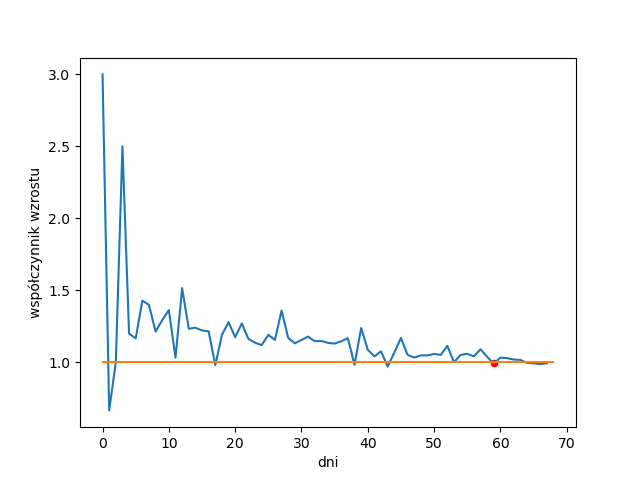
\includegraphics[width=0.8\textwidth]{Figure_1}
 \caption{Zgony} 
 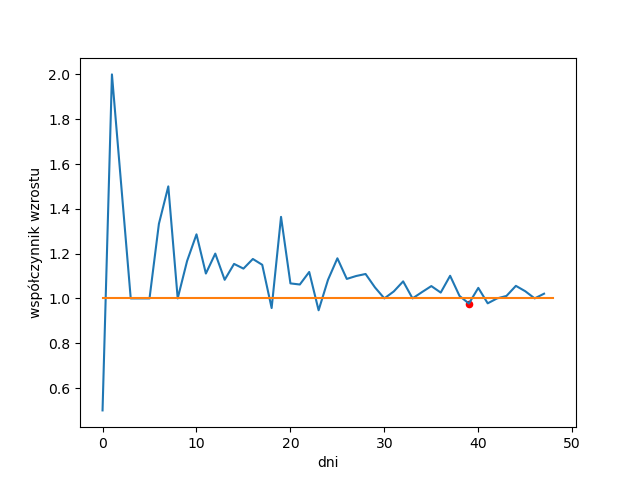
\includegraphics[width=0.8\textwidth]{Figure_2}
 \begin{flushleft}
 \end{flushleft} 
\end{figure}

\begin{figure}[hbt!]
\centering Stany Zjednoczone. Współczynnik wzrostu
 \centering
 \caption{Zachorowania}
 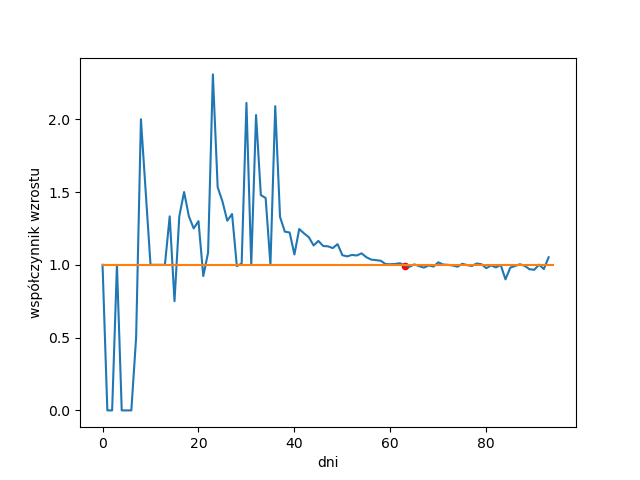
\includegraphics[width=0.8\textwidth]{Figure_3}
 \caption{Zgony} 
 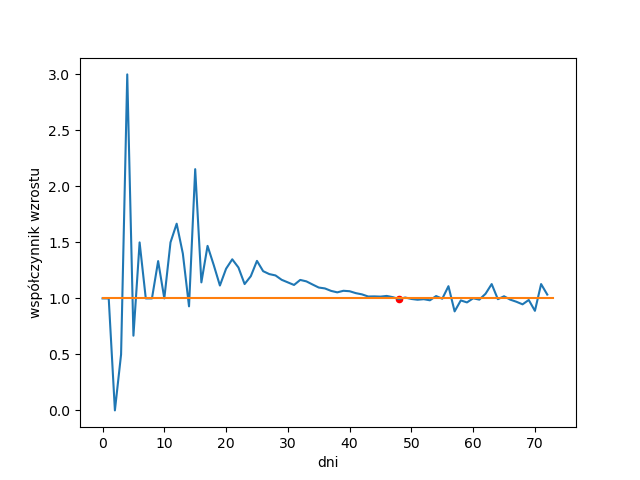
\includegraphics[width=0.8\textwidth]{Figure_4}
 \begin{flushleft}
 \end{flushleft} 
\end{figure}

\begin{figure}[hbt!]
\centering Rosja
 \centering
 \caption{Zachorowania. Dzień 2020-05-11}
 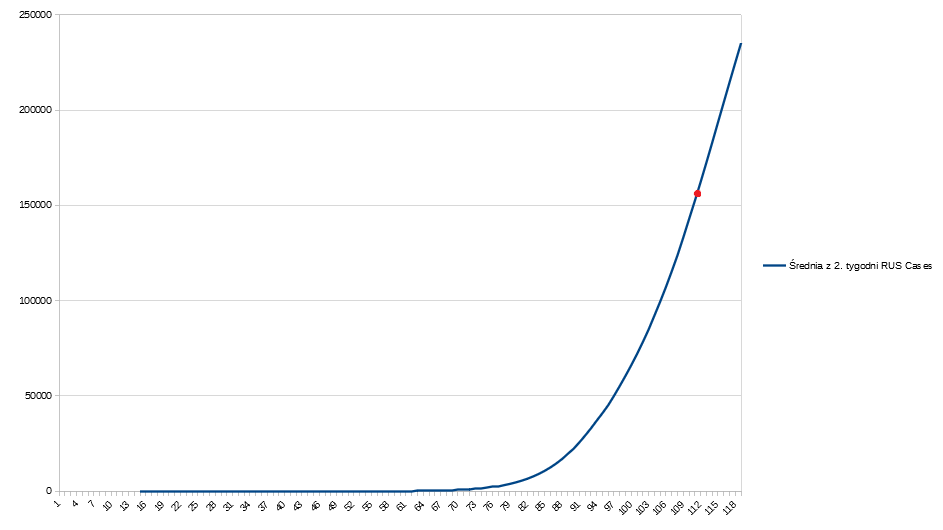
\includegraphics[width=1\textwidth]{graph1}
 \caption{Zgony. Dzień 2020-05-11} 
 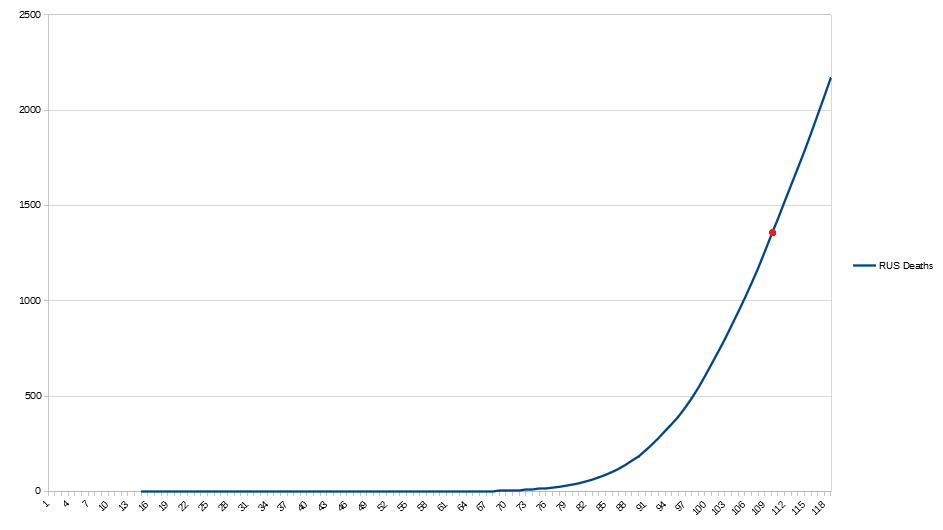
\includegraphics[width=1\textwidth]{graph2}
 \begin{flushleft}
 \end{flushleft} 
\end{figure}

\begin{figure}[hbt!]
\centering Stany Zjednoczone. 
 \centering
 \caption{Zachorowania. Dzień 2020-04-19}
 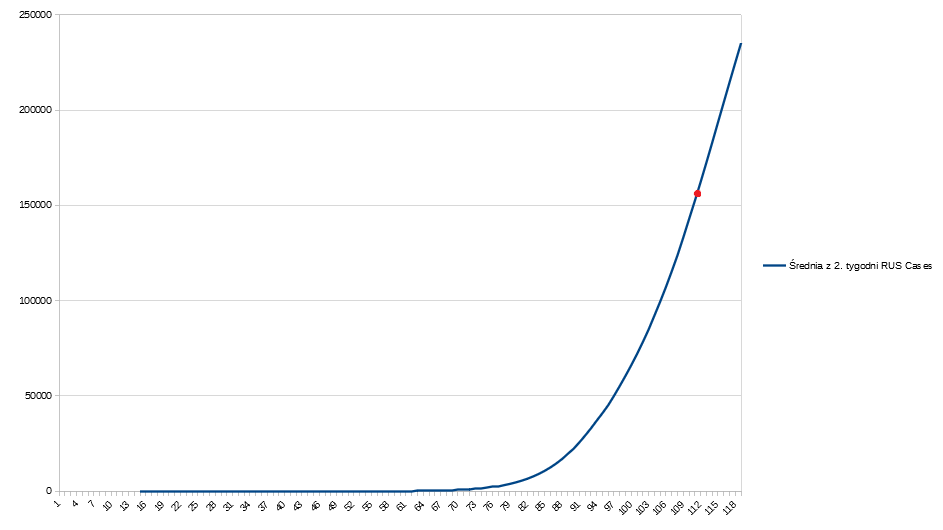
\includegraphics[width=1\textwidth]{graph1}
 \caption{Zgony. Dzień 2020-04-25} 
 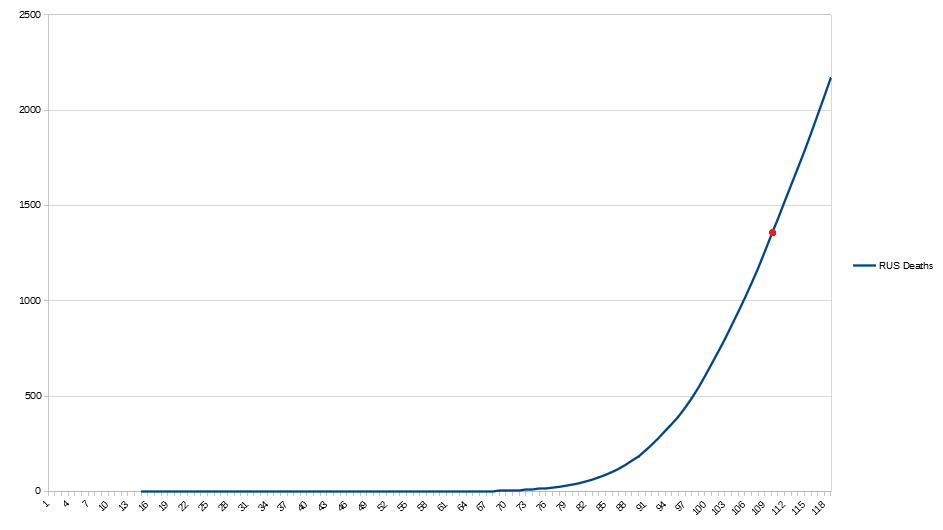
\includegraphics[width=1\textwidth]{graph2}
 \begin{flushleft}
 \end{flushleft} 
\end{figure}


\end{document}
